\documentclass[a4paper,14pt]{extreport}

\usepackage[unicode,hidelinks]{hyperref}
\usepackage[T2A]{fontenc}
\usepackage[utf8]{inputenc}
\usepackage[english,russian]{babel}
\usepackage{amsmath,amsthm,amssymb,amsfonts,mathtext,cite,enumerate,float}
\usepackage[pdftex]{graphicx}
\graphicspath{{images/}}
\usepackage{fix-cm}
\usepackage{lastpage}

\makeatletter
\renewcommand{\@biblabel}[1]{#1.}
\makeatother

\usepackage{geometry}  % Меняем поля страницы
\geometry{left=2cm}    % левое поле
\geometry{right=1.5cm} % правое поле
\geometry{top=2cm}     % верхнее поле
\geometry{bottom=2cm}  % нижнее поле

\newcommand{\HRule}{\rule{\linewidth}{0.5mm}}

\usepackage{indentfirst}
\setlength\parindent{5ex}

\usepackage{titlesec}

\titleformat{\chapter}[block]
  {\filcenter}
  {\thechapter}
  {1em}
  {\MakeUppercase}{}

\titlespacing*{\chapter}{0pt}{-30pt}{*4}

\titleformat{\section}
  {}
  {\thesection}
  {1ex}{}

\titlespacing*{\section}{\parindent}{*4}{*4}

\newcommand\chap[1]{%
  \chapter*{#1}%
  \addcontentsline{toc}{chapter}{#1}}
% Add chapter to toc

\addto{\captionsrussian}{\renewcommand*{\contentsname}{Содержание}}

\renewcommand{\theenumi}{\arabic{enumi}}                                       % Меняем везде перечисления на цифра.цифра
\renewcommand{\labelenumi}{\arabic{enumi}}                                     % Меняем везде перечисления на цифра.цифра
\renewcommand{\theenumii}{.\arabic{enumii}}                                    % Меняем везде перечисления на цифра.цифра
\renewcommand{\labelenumii}{\arabic{enumi}.\arabic{enumii}.}                   % Меняем везде перечисления на цифра.цифра
\renewcommand{\theenumiii}{.\arabic{enumiii}}                                  % Меняем везде перечисления на цифра.цифра
\renewcommand{\labelenumiii}{\arabic{enumi}.\arabic{enumii}.\arabic{enumiii}.} % Меняем везде перечисления на цифра.цифра

% \usepackage{enumitem}
% \makeatletter
    % \AddEnumerateCounter{\asbuk}{\@asbuk}{ю)}
% \makeatother
% \setlist{nosep, leftmargin=\parindent}

%  маркированные списки
\renewcommand{\labelitemi}{--}
\renewcommand{\labelitemii}{--}
%  нумерованные списки
\renewcommand{\labelenumi}{\asbuk{enumi})}
\renewcommand{\labelenumii}{\arabic{enumii})}



\theoremstyle{plain}
\newtheorem{theorem}{Теорема}[section]
\newtheorem{lemma}[theorem]{Лемма}
\theoremstyle{definition}
\newtheorem{definition}{Определение}
\theoremstyle{remark}
\newtheorem*{example}{Пример}
\newtheorem*{remark}{Замечание}




\begin{document}
  \begin{titlepage}
  \begin{center}
    Министерство общего и профессионального образования\\
    Российской Федерации \\[1em]

    НАЦИОНАЛЬНЫЙ ИССЛЕДОВАТЕЛЬСКИЙ ЯДЕРНЫЙ\\
    УНИВЕРСИТЕТ ``МИФИ'' \\[1em]

    \begin{minipage}{\textwidth}
      \begin{flushleft}
        \begin{tabular}{ l l }
          Факультет & Кибернетики и информационной безопасности\\
          Кафедра   & Информационные технологии в социальных системах
        \end{tabular}
      \end{flushleft}
    \end{minipage}\\[1em]

    \begin{minipage}{\textwidth}
      \begin{flushright}
        \textit{К защите допустить:}\\
        Заведующий кафедрой\\
        \underline{\hspace*{4.5cm}} М.\,В.~Сергиевский
      \end{flushright}
    \end{minipage}\\[3em]

    {ПОЯСНИТЕЛЬНАЯ ЗАПИСКА}\\
    {к курсовому проекту}\\
    {на тему:}\\[1em]
    \textbf{РАЗРАБОТКА АЛГОРИТМА ДЛЯ ВЫДЕЛЕНИЯ ЧАСТОВСТРЕЧАЮЩИХСЯ ШАБЛОНОВ
      ОШИБОК ИЗ ФАЙЛОВ ЖУРНАЛОВ ПРИЛОЖЕНИЙ}\\[1em]


    % {БГУИР ДП \textbf{1-31 03 04 07 093} ПЗ}\\[2em]
    \vfill

    \begin{tabular}{ p{0.65\textwidth}p{0.25\textwidth} }

      Студент: & А.\,Г.~Тропин \\

      \vfill
      Научный руководитель:\\
      к.т.н, доцент & М.\,В.~Сергиевский \\
      % Консультанты: &\\
      % \hspace*{3ex}\emph{от кафедры информатики} & А.\,А.~Волосевич \\
      % \hspace*{3ex}\emph{по экономической части} & А.\,В.~Рябов \\
      % \hspace*{3ex}\emph{по охране труда} & Е.\,А.~Колосова \\
      & \\
    \end{tabular}
    \vfill
    {\normalsize Москва 2015}
  \end{center}
\end{titlepage}





  \chap{Реферат}
  \addtocounter{page}{1}
Пояснительная записка к учебно-исследовательской работе содержит
\pageref{LastPage} страниц, 843 строки исходного кода, находящегося в откром
доступе, 2 рисунка, 5 приложений.\\

Ключевые слова: mapreduce, logs, распределенные вычисления, python, надежность,
отказоустойчивость, функциональное программирование, регулярные выражения.\\

Цель работы --- разработка алгоритма для выделения частовстречающихся шаблонов
ошибок из файлов журналов приложений для повышения скорости реакции
на непредвиденные ситуации и повышения стабильности работы распределенной
системы.

В процессе работы осуществлялась разработка алгоритма, реализация алгоритма на
языке python. И внедрение в производство с использованием MapRedcue-системы
Yandex Tables.

В результате работы был разработан алгоритм, реализован на языке
python и написаны вспомогательная утилита на языке bash и две утилиты
на языке python.




  \tableofcontents

  \chap{Нормативные ссылки}
  В настоящей пояснительной записке к учебно-исследовательской работе
использованы ссылки на следующие стандарты.\\

\href{http://nauka.kz/upload/files/17._GOST_7.32-2001.pdf}{ГОСТ 7.32-2001}
Система стандартов по информации, библиотечному и издательскому делу. Отчет о
научно-исследовательской работе. Структура и правила оформления.\\

\href{http://nauka.kz/upload/files/05._GOST_7.9-95.pdf}{ГОСТ 7.9-95}
Система стандартов по информации, библиотечному издательскому делу. Реферат
и аннотация. Общие требования.

  \chap{Определения, обозначения и сокращения}
  \begin{definition}[MapReduce]
  Модель распределённых вычислений, представленная
  компанией Google, используемая для параллельных вычислений над очень
  большими, несколько петабайт, наборами данных в компьютерных кластерах.
\end{definition}

\begin{definition}[Map]
  map(f, list) --- функция высшего порядка двух аргументов, применяет к каждому
  элементу списка list, функцию f(x), в качестве результата возвращает список
  полученных значений.
\end{definition}

\begin{example}
  map(lambda x: x**3, [1, 2, 3]) вернёт список [1, 8, 27].
\end{example}

\begin{definition}[Reduce]
  reduce(f, list, init=None) --- функция высшего порядка, последовательно
  применяет f(x, y) к элементу списка и значению от предыдущего выполнения
  функции.
\end{definition}

\begin{example}
  reduce(lambda x, y: x + y, [1, 2, 3]) вернёт 6(сумма всех элементов).
  6~=~sum(sum(1,~2),~3).
\end{example}

\begin{definition}[Экземпляр]
  Приложение, запущенное в контейнере и описываемое парой host:port.
\end{definition}

\begin{definition}[Шаблон]
  Специально подготовленное регулярное выбражение с экранированными
  спецсимволами.
\end{definition}

\begin{definition}[Эвристический алгоритм (эвристика)]
  Алгоритм решения задачи, не имеющий строгого обоснования, но, тем не менее,
  дающий приемлемое решение задачи в большинстве практически значимых случаев.
\end{definition}



  \chap{Введение}
  Большинство программных систем, имеющих сложную структуру и состоящих из нескольких сотен различных компонент(балансеры, верхние, средние метапоиски, промежуточные и базовые поиски, колдунщики, антироботы, свежесть, региональные поиск, несколько десятков параллельных поисков) обладают рядом схожих проблем. Напимер веб-поиск. Краткое схематичное описание архитектуры:

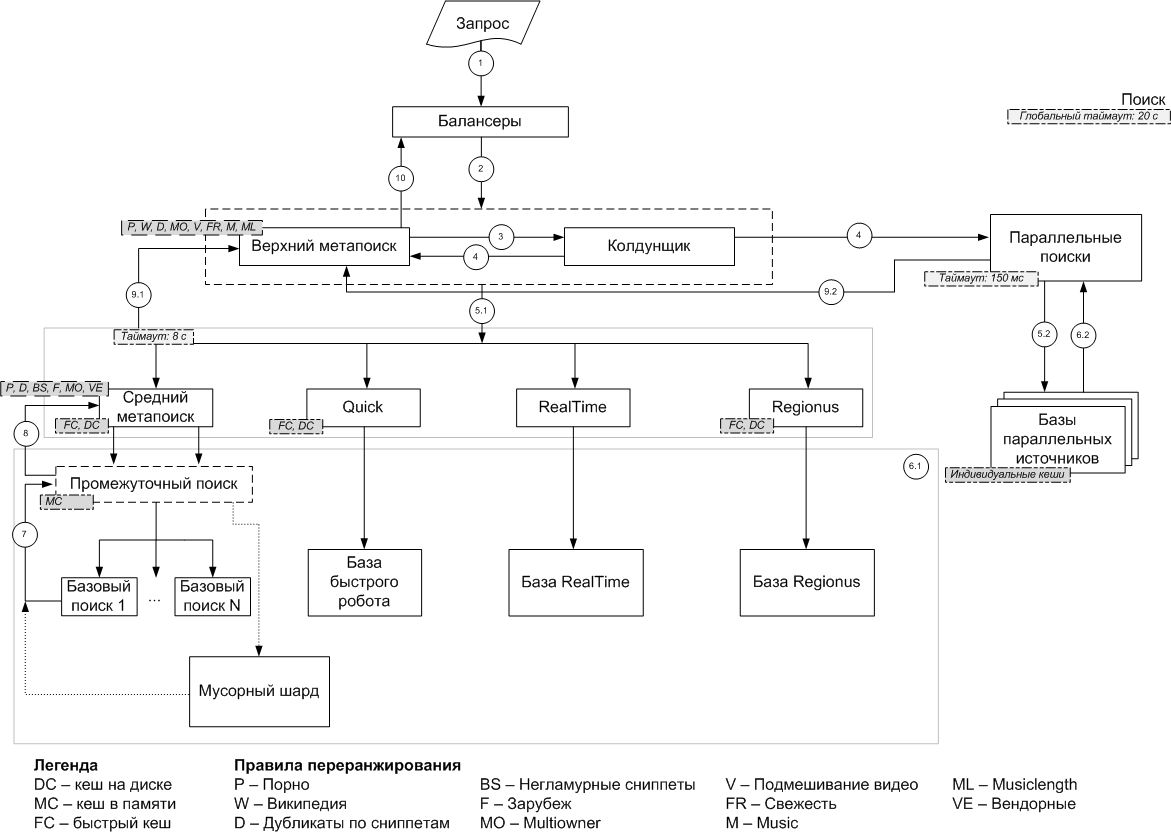
\includegraphics[width=\textwidth]{pics/search.png}

Всего единовременно запущено несколько ******** тысяч приложений. Каждое приложение генерирует множество ошибок и записывает каждую из них в log-файл.
Некоторые приложения, близкие по функционалу, пишут в один и тот же файл. Log-файлы ротируются согласно определённому алгоритму. Тем не менее объем log-файла для одного инстанса приложения может достигать нескольких сотен мегабайт, что препятствует быстрому ручному анализу в случае инцидента и инженеры вынуждены тратить ценные секунды на просмотр сотен тысяч строк файла в поисках сообщения с описанием элемента, вызвавшего сбой работы системы.

Начальным требованием к системе для эффективного использования алгоритма является наличие сопоставимого с количеством поисковых приложений количества нод на которых может быть запущена программа, реализующая алгоритм.

В организации, в которой выполнялась учебно-исследовательская работа, развернута большая поисковая инфраструктура, которая не лишена недостатков и существует вероятность поломки некоторой её части. Существует множество средств мониторинга состояния веб-поиска и противодействия инцидентам, но в некоторых случаях инженерам их недостаточно и приходится вручную анализировать log-файлы отдельных инстансов приложений на отдельных host'ах, что, в свою очередь, замедляет скорость реакции на непредвиденную ситуацию. Но даже автоматизация процесса анализа log-файла на одного инстанса не решает проблему полностью, поэтому необходима возможность быстрого анализа log-файлов сразу множества инстансов.

Таким образом, целью этой учебно-исследовательской работы является разработка алгоритма, позволяющего собирать статистику по ошибкам, встречающимся в log-файлах инстансов поисковых приложений на основе существующих шаблонов и выделять новые шаблоны.

  \chapter{Анализ предметной области}
  
\section{Актуальность задачи}
\section{Сравнение с существующими аналогами}
\section{Постановка задачи}

% \section{Представление задачи в терминах MapReduce}
% Для параллельного запуска приложений была выбрана модель распределённых
% вычислений MapReduce по ряду причин. Основные понятия:

% Как оказалось задача без особых сложностей выражается в терминах
% чистых функций flat map и flat reduce, так как основная структура,
% используемая в алгоритме --- это пара(шаблон, количество совпадений)
% и благодаря этому однопоточный код легко запускается
% на множестве узлов MapReduce-кластера. Это обстоятельство освобождает
% от реализации сложного механизма сетевого взаимодействия.

% В качестве реализации модели MapReduce была выбрана реализация
% Yandex Tables, обладающая рядом отличий и нововведений:
% \begin{itemize}
  % \item Колоночное хранение и range-операции
  % \item Дерево метаинформации
  % \item Единая операция Map-Reduce
  % \item Расширенная поддержка транзакций, включая вложенность
  % \item Настраиваемый коэффициент репликации и алгоритмы сжатия данных
  % \item Хранение файлов в системе и их раздача исполняемым задачам
  % \item Разные форматы стриминга (yamr, dsv)
  % \item Надёжность и производительность
    % \begin{itemize}
      % \item Отказоустойчивый мультимастер
      % \item Отказоустойчивый реплицированный планировщик
      % \item Минорные обновления проходят без заметного эффекта для
        % конечных пользователей
    % \end{itemize}
  % \item Гибкие слоты (заказ CPU, RAM)
  % \item Существенные обновления не требуют пересборки C++ клиентов
    % (так как все работает через HTTP API и стриминг клиент)
% \end{itemize}
% Не смотря на существенные отличия от модели, описанной в документе от компании
% Google, код программы, реализующий алгоритм легко переносится
% на другие реализации данной модели распределённых вычислений.


% \section{Выбор языка программирования и средств разработки}
% В качестве среды разработки было решено использовать удалённую виртуальную
% машину с конфигурацией и окружением идентичными конфигурации и окружению
% MapReduce узла. Были выбраны следующие программные продукты:

% \begin{itemize}

% \item В качестве операционной системы использовался дистрибутив GNU/Linux
  % Ubuntu 12.04 LTS с модифицированным ядром и дополнительными пакетами.

% \item Vim --- один из немногих настоящих текстовых редакторов,
  % обладающих массой встроенных возможностей и практически безграничным
  % потенциалом к расширению за счёт встроенного интерпретируемого языка
  % программирования VimL и поддержкой возможности написания расширений на
  % таких языках, как python, ruby, perl.

% \item Сохранение состояние рабочего окружения осуществлялось с помощью
  % терминального мультиплексора tmux, имеющего клиент-серверную архитектуру и
  % позволяющего отсоединятся от текущей сессии, оставляя её работать в фоновом
  % режиме с последующей возможностью переподключения.
  % tmux --- свободная консольная утилита-мультиплексор,
  % предоставляющая пользователю доступ к нескольким терминалам в рамках
  % одного экрана. tmux может быть отключён от экрана: в этом случае он
  % продолжит исполняться в фоновом режиме; имеется возможность вновь
  % подключиться к tmux, находящемуся в фоне. tmux является штатным
  % мультиплексором терминалов операционной системы OpenBSD.
  % Программа tmux задумывалась как замена программы GNU Screen.

% \item Удалённое подключение осуществлялось средствами защищённого протокола
% ssh\\
% (беспарольная аутентификация с использованием ключа) и технологии cauth.
% SSH (англ. Secure Shell --- ``безопасная оболочка'']) --- сетевой протокол
% прикладного уровня, позволяющий производить удалённое управление операционной
% системой и туннелирование TCP-соединений (например, для передачи файлов).
% Схож по функциональности с протоколами Telnet и rlogin, но, в отличие от них,
% шифрует весь трафик, включая и передаваемые пароли. SSH допускает выбор
% различных алгоритмов шифрования. SSH-клиенты и SSH-серверы доступны для
% большинства сетевых операционных систем.

% \item Для управления версиями исходных кодов использовалась децентрализованная
  % система управления версиями git, в качестве сервиса для хранения репозитория
  % был использован сервис github.

% \end{itemize}

% В качестве языка программирования был выбран python2.7. Так как:

% \begin{itemize}
% \item Он предустановлен в большинстве современных дистрибутивах
  % операционных систем.
% \item Выразителен. Аналогичные программы на таких языках как Java, C++
  % имеют в разы большие объёмы исходных кодов.
% \item Обладает высокой производительностью.
% \item Имеет множество библиотек, в том числе библиотеки для работы с
  % регулярными выражениями, обёртки для MapReduce.

% \end{itemize}

% \section{Структура данных}
% В качестве входных данных использовался агрегированный файл журнала с
% нерегулярной структурой, содержащий сообщения об ошибках в различных форматах,
% как многострочные, так и однострочные.

% Первая часть алгоритма, позволяет осуществить сбор статистики
% и возвращает список пар (шаблон, количество совпадений), так же существует
% возможность получить часть текста не удовлетворяющую известным шаблонам,
% для последующего анализа с помощью второй части алгоритма, позволяющей
% выделить новые предполагаемые шаблоны и с помощью первой части алгоритма
% получить статистику, подтверждающую или опровергающую предположение.

% \section{Стадии выполнения задачи}
% \subsection{Подготовка репозитория}
% Был создан git-репозиторий на сервисе github, сделана его локальная копия.
% Была выбрана следующая структура проекта и правила именования файлов:

% \begin{itemize}
% \item В корневом каталоге лежат файлы README.md, LICENSE, .gitignore.
% \item В каталоге doc/ хранится документация. Исходные тексты в \LaTeX и
  % скомпилированная версия в PDF.
% \item В каталоге direlog/ хранятся исходные коды с расширением .py и тесты,
  % имеющие префикс test\_
% \item В каталоге direlog/example/ хранятся примеры файлов журналов и
  % вспомогательные скрипты на языке bash.
% \end{itemize}

% \subsection{Выбор хранилища для шаблонов}
% В качестве хранилища для паттернов было решено использовать обычный файл на
% языке python, названный patterns.py и содержащий в себе два списка паттернов
% prepare\_patterns и main\_patterns, используемых на подготовительном этапе
% и на этапе сбора статистики соответственно,
% и хранить его под контролем версий в этом же репозитории. Причин
% на это несколько: во-первых простота модификации файла с помощью скриптов,
% во-вторых возможность просмотра истории изменений и откат к предыдущим версиям,
% в-третьих возможность ручного редактирования.

% \subsection{Написание программного кода}

% Для разработки приложения, реализующего алгоритм была использована одна из
% гибких методологий разработки - экстремальное программирование.\\

% Использовались следующие приёмы этой методологии разработки:

% \begin{itemize}
  % \item Короткий цикл обратной связи
    % \begin{itemize}
      % \item Разработка через тестирование
      % \item Заказчик всегда рядом
      % \item Парное программирование
    % \end{itemize}
  % \item Непрерывный, а не пакетный процесс
    % \begin{itemize}
      % \item Непрерывная интеграция
      % \item Рефакторинг
      % \item Частые небольшие релизы
    % \end{itemize}
  % \item Понимание, разделяемое всеми
    % \begin{itemize}
      % \item Простота
      % \item Коллективное владение кодом
      % \item Стандарт кодирования
    % \end{itemize}
    % \item Социальная защищённость программиста
      % \begin{itemize}
        % \item 40-часовая рабочая неделя
      % \end{itemize}
% \end{itemize}

% В результате можно выделить следующие этапы развития приложения:\\

% \begin{enumerate}
% \item Написание функциональных тестов для prepare.py.
% \item Написание утилиты для предварительной обработки исходного файла журнала.
  % Утилита получила название prepare.py и позволила подготовить сырой файл
  % журнала для последующей обработки, путём замены уникальных токенов, таких
  % как UUID, timestamp, версии, номера строк, пути, содержащие версии, на
  % строковые константы.
% \item Формирование prepare\_patterns на основе ручного анализа
  % файлов журналов.
% \item Написание функциональных тестов для direlog.py.
% \item Реализация алгоритма для сбора статистики с использованием
  % main\_patterns. Утилита получила название direlog.py. И позволяет на
  % выходе получить список пар (шаблон, количество совпадений) или текст,
  % не подходящий под известные шаблон.
% \item Написание функциональных тестов для direlog.py.
% \item Добавление поддержки буферизации входного потока и поддержки
  % многострочных шаблонов.
% \item Добавление функции, позволяющей запускать алгоритм на MapRedcue-кластере.
% \end{enumerate}



  \chapter{Имплементация задачи}
  \section{Диаграмма компонентов}
  \section{Описание способов запуска}
  % Структурная схема приложения питонячие файлики, тесты, примеры логов.
  % как запускаются, как работают.
  \section{Анализ полученных результатов}
  % Что получил

  \section{Дальнейшее развитие}
  % Автоматическое выделение паттернов. Итерационная схема с эвристикой.
  % Интеграция с другими программными продуктами.



  \chap{Заключение}
  % Делали, сделали за пол года такой кусок, есть план на следующий год.

  \chap{Список использованных источников}
  \chap{Приложения}
  % \part{}
  %\input{ch1}

\end{document}

